\chapter{Methodology}

\begin{figure}[htp]
    \centering
    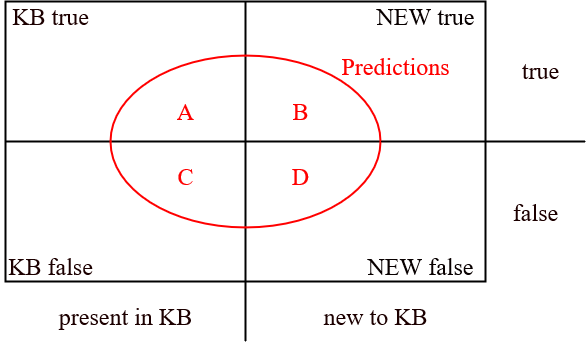
\includegraphics[width=10cm]{figures/kb_venn.png}
    \caption{KB prediction under incompleteness}
\end{figure}

\begin{figure}[htp]
    \centering
    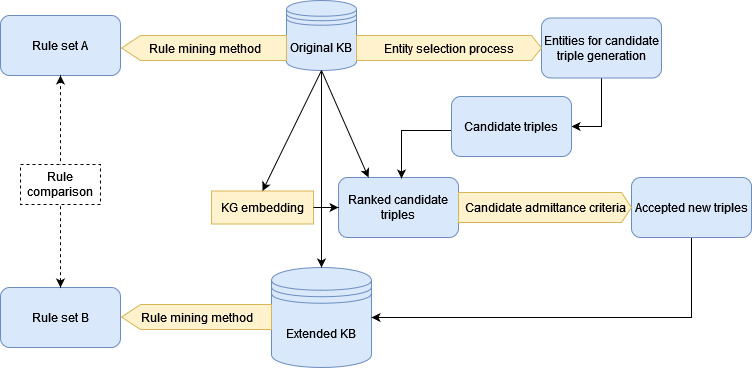
\includegraphics[width=12cm]{figures/ontology_mining_pipeline.jpg}
    \caption{KB prediction under incompleteness}
\end{figure}


\section{Knowledge Graph Datasets}
While there are many large KGs publicly available, they are often quite complex in the number of different relations and entities used. Since we are mining rules over relations, the relational aspect of the KGs used was kept simple. By limiting the number of relations used in the KGs the resulting rules mined won't be overly diverse, and therefore easier for a human to understand evaluate. Two different datasets were used to conduct the experiments, both of which had been limited to contain only six different types of relations.


\subsection{Wikidata5M - family KG}
Wikidata5M is a KG dataset containing over 20 million triples with over 800 types of relations. It combines information from the Wikidata KG with Wikipedia pages \cite{wang2019kepler}. Wikidata5M uses the same identifier system as Wikidata, where each entity and relation is assigned a unique ID. The IDs of entities are prefixed with \texttt{Q} and those of relations with \texttt{P}. For example the following line \\
\centerline{\texttt{\href{https://www.wikidata.org/wiki/Q146}{Q146} \quad \href{https://www.wikidata.org/wiki/Property:P279}{P279} \quad  \href{https://www.wikidata.org/wiki/Q39201}{Q39201}}} \
corresponds to \textless\texttt{\href{https://www.wikidata.org/wiki/Q146}{house cat}, \href{https://www.wikidata.org/wiki/Property:P279}{subclass of}, \href{https://www.wikidata.org/wiki/Q39201}{pet}}\textgreater, where each entity has a corresponding Wikipedia page.
This dataset was chosen due to its size and because it contained family-related information. Rules about family structure are well-known and easy to comprehend. For example the simple rule $parent(a, b) \Rightarrow  child(b, a)$ would be implicitly represented in the data of such a subset.
\begin{lstlisting}[language=Python, caption={Python dictionary converting family predicate IDs to their names},captionpos=t, label={family_predicated_dict}]
family_predicates_dict = {
    'P40': 'child', 
    'P22' : 'father', 
    'P25' : 'mother',
    'P26' : 'spouse', 
    'P1038' : 'relative', 
    'P3373' : 'sibling', 
}
\end{lstlisting}

After filtering out all triples that did not use one of the six selected family predicates, the IDs were converted to meaningful names so that the resulting rules mined would be easily readable. The python dictionary listen in \ref{family_predicated_dict} shows the chosen predicates. A few other family predicates were considered, but did not have as many corresponding data points or were too similar to other selected predicates. Predicates such as \texttt{grandchild} or \texttt{sister} are also not currently used in Wikidata, and from a discussion in the Wikidata community it seems that all properties considered redundant were removed \cite{kinship_discussion}. For the experiments Pykeen's distribution of the dataset was used \cite{ali2021pykeen}. The resulting subset of Wikidata5M contained around 250 000 triples and will henceforth be refferred to as the \textit{family KG}. 

\subsection{WN18RR}
WN18RR is a smaller KG dataset with 93 003 triples and only 11 relations \cite{dettmers2018convolutional}. It is based on the WN18 dataset, which contains triples scraped from WordNet, a lexical database for English \cite{wordNet}. It was found that there was information leakage between the training and test set of WN18 through inverse relations, where a large number of test triples could be identified simply by inverting triples in the training set \cite{toutanova2015observed}. WN18RR addresses this issue. In WordNet nouns, verbs, adjectives and adverbs are grouped into sets of semantic synonyms called \textit{synsets}. An example if a synset is \textit{\textbf{cat, true cat} (feline mammal usually having thick soft fur and no ability to roar)}. Synsets are connected to other synsets by semantic relations. The most commonly used relation in WN18RR is \texttt{hypernym}. A synset \texttt{X} is a hypernym of synset \texttt{Y}, if every \texttt{Y} is a kind of \texttt{X}. For example the triple 
\centerline{\texttt{02121808 \quad hypernym \quad 02121620}}
represents the information that the synset \texttt{cat} is a hypernym of the synset \texttt{house cat}. Or more simply phrased: \textit{All house cats are cats}.

\begin{table}[ht]
\centering
\begin{tabular}{|c|c|c|}
\hline
& \textbf{Relation} & \textbf{Frequency}\\
\hline
\multirow{6}{*}{\rotatebox[origin=c]{90}{Included}} &hypernym & 36873\\
&derivationally related form & 31865\\
&member meronym & 7912\\
&has part & 5131\\
&synset domain topic of & 3328\\
&instance hypernym & 3118\\
\hline
\multirow{5}{*}{\rotatebox[origin=c]{90}{Not included}}&also see & 1396\\
&verb group & 1220\\
&member of domain region & 981\\
&member of domain usage & 673\\
&similar to & 86\\
\hline
\end{tabular}
\caption{Frequency of relations in WN18RR KG and whether they were included in the final KG}
\end{table}

WN18RR was chosen because the number of relations needed to be limited, and with a dataset already containing few relations most of it could be included. By taking all triples containing one of the six most frequent relations, in total 88227 datapoints, 95\% of WN18RR was used. This was intended to produce a more complete KG.

\section{Model selection}


\section{Candidate generation and ranking}



\section{Rule mining and evaluation}
